\documentclass[line, margin]{res}
\usepackage{CJK}
\usepackage{url}
\usepackage{graphicx}
\usepackage{wrapfig}

\begin{document}
%\begin{CJK}{GBK}{kai}


\name{Xian Yang}

%\name{����}
\address{No.398 Ruoshui street, industrial district, Suzhou}
\address{yangxian10@gmail.com \\ 15952446119}

\begin{wrapfigure}{r}{0\textwidth} %this figure will be at the right
\centering
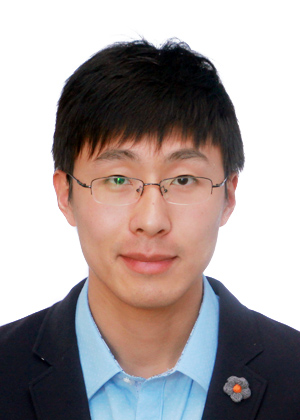
\includegraphics[width=0.18\linewidth]{yang.jpg}
\end{wrapfigure}

%\begin{figure}[!h]
%\raggedleft
%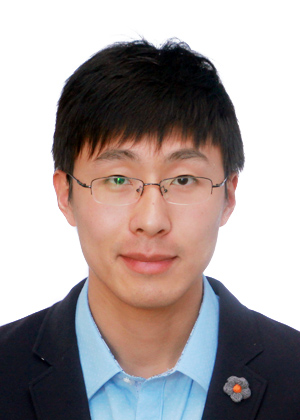
\includegraphics[width=0.18\textwidth]{yang.jpg}
%\end{figure}

\begin{resume}


\section{JOB OBJECTIVE}
\textbf{: Analytics Specialist}

\section{EDUCATION}
%\begin{tabular}{l l l l}
 2010.9 - Present  \textbf{Institute of Semiconductor, CAS} \\
 Doctor of Microelectronics and Solid State Electronics\\

 2006.9 - 2010.7  \textbf{Xidian University}\\
 Bachelor of Applied physics, ranking 1/80
%\end{tabular}

\section{SKILLS}
\begin{itemize}
\item IT skills: \textbf{C/C++}, \textbf{python}, \textbf{matlab}
\item Open source tools: \textbf{OpenCV}, \textbf{scikit-learn}
\item Research interests: \textbf{machine learning, pattern recognition, computer vision},\textbf{unspecified visual object tracking}
\item Techblog: \url{http://blog.csdn.net/yang_xian521} Page View: \textbf{810,000}
\item CET-6 Pass, excellent reading and writing, basic spoken English
\end{itemize}

\section{EXPERIENCE}
\textbf{Wave Group Intelligent active security R\&D center} \hfill 2012.3-2014.4 \\
\begin{itemize}
\item Design and optimize unspecified visual object tracking independently, implement dynamic background unspecified object tracking robustly and publish articles.
\item Participate in designing and discussion of single sample person recognition, and achieve 93\% recognition rate in the actual conditions.
\end{itemize}

\textbf{National Undergraduate Electronic Design Contest} \hfill 2009.4-2009.9 \\
\begin{itemize}
\item Lead a three-person team, assign task, take part in internal training and competition
\item Make more than ten electronic modules such as switched-mode power supply, audio power amplifier and CNC obstacle avoidance car, involved a wide range of knowledge such as Digital signal processing, Microcontroller programming and Analog electronic circuit design.
\item In four days of the match, we designed and implemented a digital filter with MCU and FPGA. I designed the organizational scheme and arranged the tasks of each stage.
\end{itemize}

\section{HONORS}
\begin{tabular}{l l l}
Academic�� & 2009 & \textbf{\textit{National Scholarship}(1\%)} \\ [5pt]
 & 2009 & \textbf{\textit{NUEDC Shanxi provincial second prize}} \\ [5pt]
 & 2008 & \textit{Outstanding students pacesetter cadres} \\ [10pt]
Community�� & 2010 & \textbf{\textit{Graduate for outstanding student cadres}(1\%)} \\ [5pt]
 & 2011 & \textbf{\textit{Merit student of CAS.}(2\%)} \\ [5pt]
 & 2007,2009 & \textit{Excellent cyl cadres} \\ [5pt]
 & 2013 & \textit{Outstanding volunteers} \\ [10pt]
Sports�� & & \textit{Prize in the school basketball game for many times}
\end{tabular}

\end{resume}
%\end{CJK}
\end{document}
